\chapter{Introduction to GUI Programming (Tkinter)}

\section{Introduction: Real-Life Hook}

When students use:
\begin{itemize}
    \item Calculator app
    \item Mobile games
    \item Music players
\end{itemize}

They click:
\begin{itemize}
    \item Buttons
    \item Menus
    \item Text boxes
\end{itemize}

These programs do not use black screens with text.
They use \textbf{Graphical User Interface (GUI)}.

In this chapter, we will learn how to create simple GUI programs using \textbf{Tkinter}.

\section{What Is GUI?}

\begin{definition}{GUI}
GUI (Graphical User Interface) allows users to interact with programs using \textbf{windows, buttons, and icons}.
\end{definition}

GUI makes programs:
\begin{itemize}
    \item Easy to use
    \item Attractive
    \item User-friendly
\end{itemize}

\section{What Is Tkinter?}

Tkinter is:
\begin{itemize}
    \item Python’s built-in GUI library
    \item Easy for beginners
    \item Available without extra installation
\end{itemize}

\section{First GUI Window}

\begin{verbatim}
import tkinter as tk

window = tk.Tk()
window.title("My First App")
window.mainloop()
\end{verbatim}

This code:
\begin{itemize}
    \item Creates a window
    \item Keeps it open
\end{itemize}

\section{Adding a Label}

\begin{verbatim}
import tkinter as tk

window = tk.Tk()
label = tk.Label(window, text="Hello, Tkinter!")
label.pack()
window.mainloop()
\end{verbatim}

\section{Adding a Button}

\begin{verbatim}
import tkinter as tk

def say_hello():
    print("Hello Student!")

window = tk.Tk()
button = tk.Button(window, text="Click Me", command=say_hello)
button.pack()
window.mainloop()
\end{verbatim}

\section{Real-Life Example: Digital Greeting Card}

\begin{verbatim}
import tkinter as tk

def greet():
    label.config(text="Good Morning!")

window = tk.Tk()
window.title("Greeting App")

label = tk.Label(window, text="Welcome")
label.pack()

button = tk.Button(window, text="Greet", command=greet)
button.pack()

window.mainloop()
\end{verbatim}

\section{Input Using Entry Widget}

\begin{verbatim}
import tkinter as tk

def show_name():
    name = entry.get()
    label.config(text="Hello " + name)

window = tk.Tk()

entry = tk.Entry(window)
entry.pack()

label = tk.Label(window, text="")
label.pack()

button = tk.Button(window, text="Submit", command=show_name)
button.pack()

window.mainloop()
\end{verbatim}

\section{Layout Managers (Brief)}

Tkinter uses layout managers:
\begin{itemize}
    \item pack()
    \item grid()
    \item place()
\end{itemize}

For beginners, \texttt{pack()} is enough.

\section{Mini-Project: Simple Calculator (GUI)}

\begin{verbatim}
import tkinter as tk

def add():
    a = int(entry1.get())
    b = int(entry2.get())
    label.config(text=a + b)

window = tk.Tk()
window.title("Mini Calculator")

entry1 = tk.Entry(window)
entry1.pack()

entry2 = tk.Entry(window)
entry2.pack()

button = tk.Button(window, text="Add", command=add)
button.pack()

label = tk.Label(window, text="")
label.pack()

window.mainloop()
\end{verbatim}

Students learn:
\begin{itemize}
    \item GUI inputs
    \item Button actions
    \item Real application logic
\end{itemize}

\section{Diagram: GUI Components}

\begin{center}
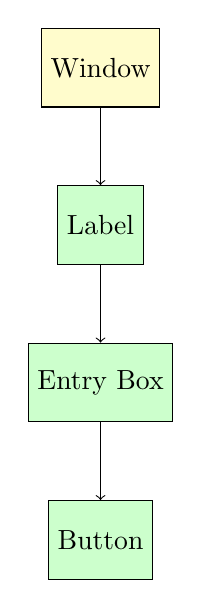
\begin{tikzpicture}[node distance=2cm]
\node (win) [draw, rectangle, fill=yellow!20, minimum height=1cm] {Window};
\node (label) [draw, rectangle, fill=green!20, below of=win, minimum height=1cm] {Label};
\node (entry) [draw, rectangle, fill=green!20, below of=label, minimum height=1cm] {Entry Box};
\node (button) [draw, rectangle, fill=green!20, below of=entry, minimum height=1cm] {Button};

\draw[->] (win) -- (label);
\draw[->] (label) -- (entry);
\draw[->] (entry) -- (button);
\end{tikzpicture}
\end{center}

\section{Why GUI Programming Is Important}

\begin{itemize}
    \item Most real apps use GUI
    \item Improves user experience
    \item Makes learning fun
\end{itemize}

\section{Key Concepts}

\begin{itemize}
    \item GUI uses windows and buttons
    \item Tkinter is Python’s GUI library
    \item Widgets build interface
    \item Events connect actions
\end{itemize}

\section{Common Beginner Mistakes}

\begin{itemize}
    \item Forgetting \texttt{mainloop()}
    \item Mixing layout managers
    \item Not handling input errors
\end{itemize}

\section{End-of-Chapter Exercises}

\subsection{Very Short Questions}

\begin{enumerate}
    \item What does GUI stand for?
    \item What is Tkinter?
    \item Name any two Tkinter widgets.
\end{enumerate}

\subsection{Short Answer Questions}

\begin{enumerate}
    \item Explain GUI with a real-life example.
    \item Difference between CLI and GUI.
    \item What is a widget?
\end{enumerate}

\subsection{Activity-Based Exercises}

\begin{enumerate}
    \item Create a GUI that displays your name.
    \item Design a button-based greeting app.
    \item Extend calculator to subtract numbers.
\end{enumerate}

\section{Teacher Notes}

\marginnote{
\textbf{Learning Objectives}
\begin{itemize}
    \item Students understand GUI basics
    \item Students use Tkinter widgets
    \item Students build simple applications
\end{itemize}

\textbf{Teaching Tips}
\begin{itemize}
    \item Demonstrate live GUI
    \item Compare CLI vs GUI
    \item Encourage creative layouts
\end{itemize}

\textbf{Assessment}
\begin{itemize}
    \item Functional GUI
    \item Proper event handling
\end{itemize}
}